\chapter{Finite Mean Flow Simulations}
\label{app_mean_flow}

In the main text, I focused on one particular LAPD experiment, which essentially contained no mean ${\bf E \times B}$ flow or flow shear. Focusing on this null flow experiment
allowed me to model the system with a smaller number of linear terms in the equation set than if the experiment had contained significant ${\bf E \times B}$ flow. 
Furthermore, neglecting mean flow and flow shear eliminated a couple of linear instabilities, namely Kelvin-Helmholtz
and rotational interchange instabilities, which are both flute-like ($k_{\para} = 0$) instabilities. It would have been less obvious, then, that the nonlinear instability caused the appearance
of dominant $k_{\para} = 0$ structures, though ultimately, energy analysis would have sorted this out. Furthermore, the low flow experiments have proven to be easier to successfully simulate than
the high flow experiments, and the null flow experiment and simulations contain so much interesting physics that they deserve study in their own right.

In this appendix, I review preliminary results of simulations and analysis of finite mean flow experiments recently conducted in LAPD. 
I have chosen to present this in an appendix, rather than including it in the main text because
it is preliminary work with much to still be done. Moreover, mean flow shear suppression is somewhat off topic from the pure drift wave turbulence that I studied in the main
text, and it wouldn't necessarily add to the main points that I developed there. But I cannot emphasize enough how important well-validated, well-analyzed mean flow simulations would be
to the understanding of these experiments and the important effects that they were designed to illuminate. Because of that, I present here my preliminary results of some mean flow simulations
so that others can build upon this work.


\section{The LAPD Biasing Experiment}
\label{s_biasing_exp}

\begin{figure}[!ht]
\centerline{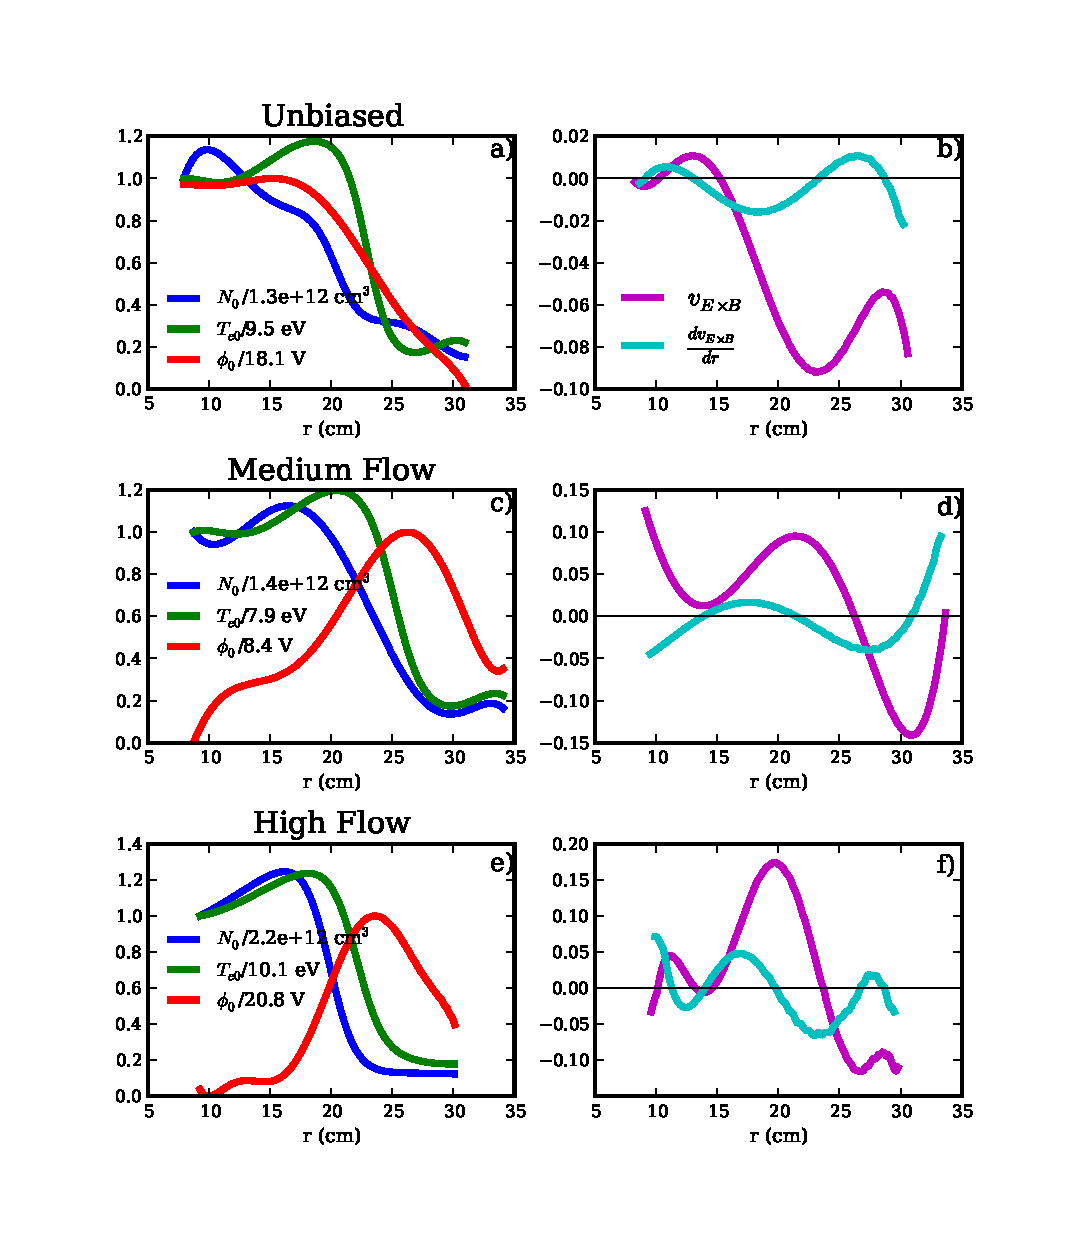
\includegraphics[]{flow_profiles}}
\caption{Equilibrium profiles for different biases}
\label{flow_profiles}
\end{figure}

The high ${\bf E \times B}$ flow and flow shear LAPD experiments are relevant to tokamak research, specifically research into the High Confinement Mode (H-mode)
and the transition to the H-mode. Researchers have long realized that H-mode is associated with strong toroidal rotation of the tokamak plasma and that the shear associated with this rotation
is the likely cause of the decrease in energy transport. The particular physical mechanism of turbulent-shear interaction that causes the flux suppression is still an area of intense
research, and many testable theories have been created to address this.

To try to answer some of the questions regarding the interaction of mean flow and flow shear on turbulence, David Schaffner, Troy Carter, and others recently set up an experiment on LAPD
in which they varied the mean flow and flow shear. In order to vary the ${\bf E \times B}$ flow, they inserted a biasable azimuthal limiter into LAPD. The limiter has radius ~26 cm, and
can be biased with respect to the cathode. When the cathode and the limiter are unbiased (maintained at the same potential), no net current flows between them, and one can imagine them
as a single conducting plate. In this case, my discussion of the sheath in Sec.~\ref{ss_bs_bc}, specifically Eq.~\ref{sheath_current}, accounts for how the plasma potential is set by
the current into the plate and the temperature profile. I considered the case for a floating conducting plate, in which, $\phi = \Lambda T_e /e$, with 
$\Lambda = \rm{ln} \left( \frac{1}{2 \sqrt{\pi}} \sqrt{\fmie}  \right)$, and where $\phi$ is the potential difference between the sheath edge and the conducting plate. If the plate is not
floating, but drawing a current, as is the case with the cathode, the proportionality factor relating $\phi$ and $T_e$ is different and not necessarily constant:

\beq
\label{lambda_r}
\Lambda(r) = \rm{ln} \left( \frac{1}{2 \sqrt{\pi}} \sqrt{\fmie} \frac{1}{1 - \frac{J_\para}{e n c_s}} \right).
\eeq
Nevertheless, the radial shape of $\phi$ somewhat mimics that of $T_e$ so long as there is no potential difference between the limiter and cathod. 
I show the equilibrium density, electron temperature, and potential profiles
for the case of the unbiased limiter in Fig.~\ref{flow_profiles} a). The potential profile, to which I have added an arbitrary constant, has the same general shape as the temperature profile,
but is somewhat different due to the weak radial dependence of $\Lambda$ in Eq.~\ref{lambda_r} due to the finite cathode current.

The situation changes when plates at different radii -- such as the cathode and the limiter -- are maintained at a different
potential and thus draw different currents. Then the proportionality function $\Lambda(r)$ becomes a stronger function of radius, and $\phi$ no longer mimics $T_e$. 
I show the equilibrium profiles when relatively
high biasing is applied in Fig.~\ref{flow_profiles} b), and when very high biasing is applied in Fig.~\ref{flow_profiles} c). Notice that the direction of the radial electric field (the radial
derivative of the potential) changes inside of the limiter radius due to the biasing. Also note that although I do not show it in Fig.~\ref{flow_profiles}, there is a level of intermediate
biasing in which the radial electric field inside of the limiter radius nulls out. In the main text, I based my simulations and analysis off of 
the profiles and turbulence realizations associated with that biasing.

An alternative way to see why the radial electric field can change due to biasing between the cathode and the limiter is to imagine the system as a circuit. The circuit runs from the limiter
through the biasing source (maintaining a potential difference) through the cathode and finally through the plasma itself, which fills the region between the cathode and the limiter.
The electrons in the plasma can carry the current along the magnetic field lines, but many of the field lines that terminate on the cathode are radially separated from the limiter field lines,
so a radial current forms to complete the circuit. This radial current is primarily carried by ions. Recall from Sec.~\ref{s_vorticity_eqn} that there are two contributions from the ions
to the cross-field current: the polarization current and the Pederson current. The radial polarization current, however, only has a time-indepdendent part due to an azimuthal electric field,
which can't be maintained due to the conducting plates. The Pederson current, however, produces a radial current through a time-independent radial electric field, so it is in fact the Pederson
current which completes the circuit and is connected with the radial electric field. Biasing then, through sheath properties and plasma currents, can change the radial potential profile.
This, of course, produces mean azimuthal ${\bf E \times B}$ flows that can have radial shear.

In the biasing experiements that are well documented in Schaffner et al.~\cite{schaffner2012,schaffner2013}, the bias voltage is changed incrementally through ~30 different values. 
The mean flow of the unbiased state points in the ion diamagnetic direction. As the bias increases, this flow nulls out and then changes direction inside of the limiter radius, which is
clear from the few instances I show in Fig.~\ref{flow_profiles}. Moreover, the radial flow shear also changes with changing bias, with the shear rate $\gamma_s$ ranging from zero to about five times
the autocorrelation time $\tau$. They find that the radial particle flux is inversely proportional to the flow shear regardless of the flow direction~\cite{schaffner2012}. 
Naturally, the density scale length is also inversely proportional to the flow shear. The experiment clearly shows that flow shear suppresses radial particle flux through suppression of turbulent
density fluctuations. 
The mechanism that causes this, however, is less obvious, and they try to answer this by comparing shear scaling properties to various theoretical predictions~\cite{schaffner2013}.
This is one instance in which simulations with highly resolved spatial features can help.

Other interesting findings in the biasing experiment include a change in the shape of the frequency spectra with flow or flow shear. As the flow and flow shear become large, a coherent feature,
seen as a sharp peak at the low end of the frequency spectra, emerges. Furthermore, the spectra become more exponential at high frequency as the flow and flow shear increase. These signal
possible changes in the nature of the turbulence. The coherent feature, for instance, indicates the presence of a coherent mode, possibly due to a flow instability. The exponential spectra,
one might speculate, might indicate a change in the chaotic properties of the turbulence, namely, a decrease in the attractor dimension. This speculation can likely be sorted out with
the help of well-validated numerical simulations. Therefore, I have attempted to simulate a few of the different biased cases and analyze the results using the tools I used in the main
text on the null flow experiment and simulations.



\section{Simulation Model}
\label{s_sim_model}

\beqar
\label{ni_eq_flow}
\pdt N = - {\mathbf v_E} \cdot \grad N_0 - {\mathbf v_{E0}} \cdot \grad N - N_0 \gradpar \vpe + \mu_N \gradperp^2 N + S_N + \{\phi,N\}, \\
\label{ve_eq_flow}
\pdt \vpe = - {\mathbf v_{E0}} \cdot \grad \vpe - \fmie \frac{T_{e0}}{N_0} \gradpar N \nonumber \\
- 1.71 \fmie \gradpar T_e + \fmie \gradpar \phi - \nue \vpe + \{\phi,\vpe \}, \\
\label{rho_eq_flow}
\pdt \varpi = - {\mathbf v_E} \cdot \grad \varpi_0 - {\mathbf v_{E0}} \cdot \grad \varpi- 
\frac{1}{r} \pdiff{\phi_0}{r} \left(\pdiff{N_0}{r} \pdiffxy{\phi}{r}{\theta} - \pdiffs{\phi_0}{r} \pdiff{N}{\theta} \right) \nonumber \\
 - N_0 \gradpar \vpe  - \nuin \varpi + \mu_\phi \gradperp^2 \varpi + \{\phi,\varpi \}, \\
\label{te_eq_flow}
\pdt T_e = - {\mathbf v_E} \cdot \grad T_{e0} - {\mathbf v_{E0}} \cdot \grad T_e - 1.71 \frac{2}{3} T_{e0} \gradpar \vpe + \frac{2}{3 N_0} \kpe \gradpar^2 T_e  \nonumber \\
- \frac{2 m_e}{m_i} \nue T_e  + \mu_T \gradperp^2 T_e +  S_T + \{\phi,T_e\}.
\eeqar

\section{New Linear Instabilities}
\label{s_flow_inst}

\section{Statistical Comparisons to Experiment}
\label{s_flow_stats}

\begin{figure}[!ht]
\centerline{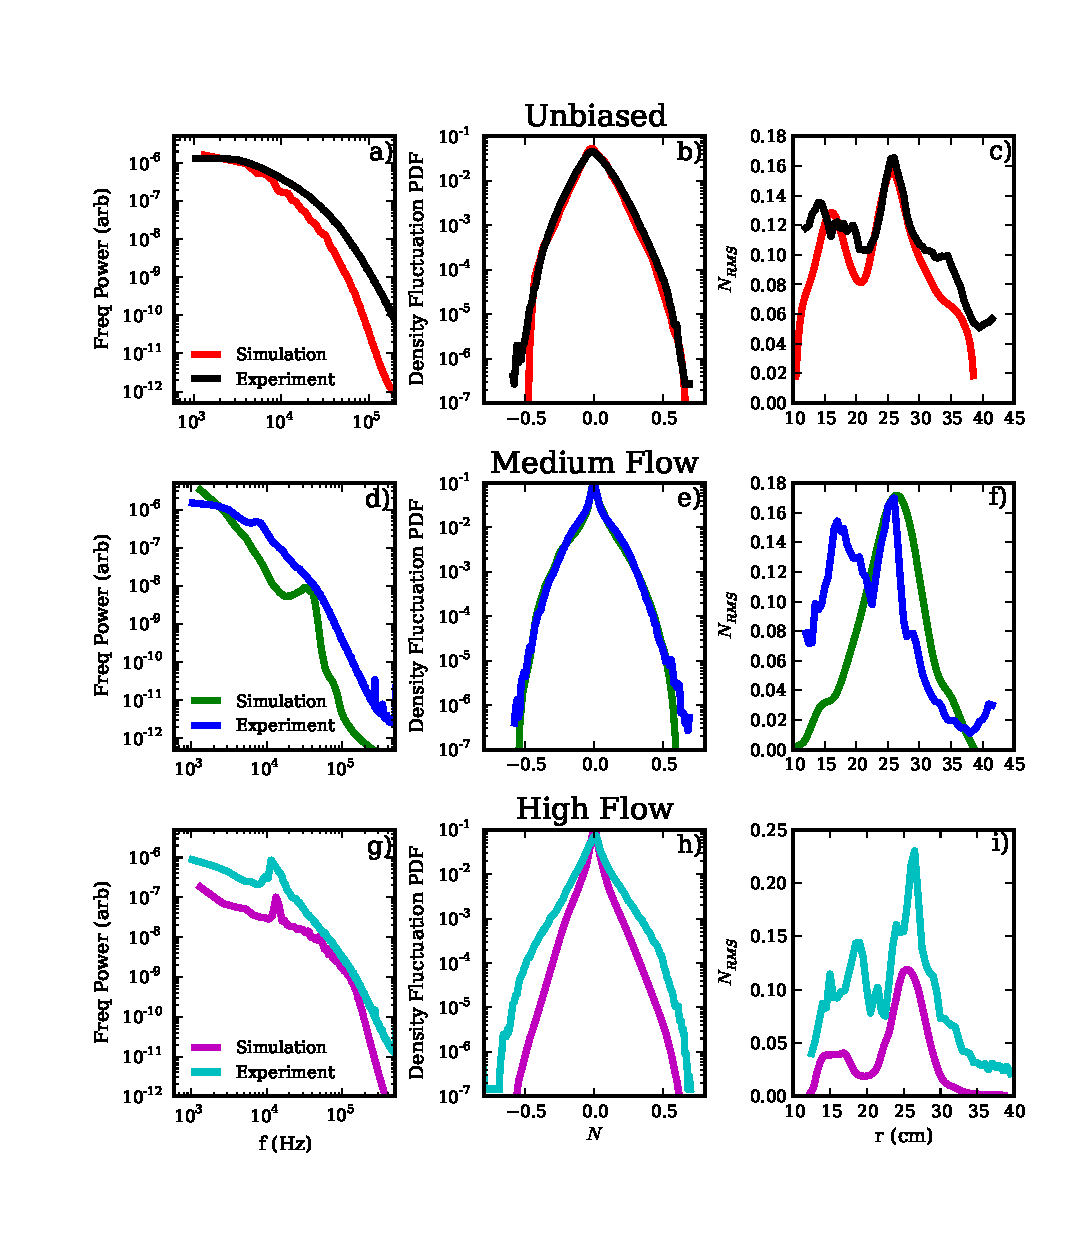
\includegraphics[]{flow_statistics}}
\caption{Mean flow experiment and simulation statistical comparisons}
\label{flow_statistics}
\end{figure}


\section{Energy Dynamics Results}
\label{s_flow_en_dyn}
